\documentclass{article}

\usepackage[a4paper, total={7.5in, 10.5in}]{geometry}
\usepackage{amsmath}
\usepackage{mathtools}

\title{Datenbanksysteme 1 - Zusammenfassung}

\usepackage{xcolor}
\usepackage{amssymb}
\usepackage{ifsym}
\usepackage{algorithm2e}
\usepackage{relsize} % for bigger mathsymbols

% syntax highlighting for java
\usepackage{listings}
\usepackage{color}
\usepackage{tikz}
\newcommand*\circled[1]{\tikz[baseline=(char.base)]{\node[shape=circle,draw,inner sep=2pt] (char) {#1};}}

\definecolor{dkgreen}{rgb}{0,0.6,0}
\definecolor{gray}{rgb}{0.5,0.5,0.5}
\definecolor{mauve}{rgb}{0.58,0,0.82}
\definecolor{black}{rgb}{0,0,0}

\lstset{frame=tb,
  language=Java,
  aboveskip=3mm,
  belowskip=3mm,
  showstringspaces=true,
  % columns=flexible,
  basicstyle={\small\ttfamily},
  numbers=left,
  numbersep=10pt,
  % showspaces=true,
  numberstyle=\tiny\color{black},
  keywordstyle=\color{blue},
  commentstyle=\color{dkgreen},
  stringstyle=\color{mauve},
  breaklines=true,
  breakatwhitespace=true,
  tabsize=4
}

\graphicspath{{images}}
\newcommand{\fullouterjoin}{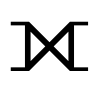
\includegraphics[scale=0.1, trim=0 1cm 0 5cm]{/full_outer_join.png}}
\newcommand{\leftouterjoin}{
\includegraphics[scale=0.05, trim=0 1.5cm 0 5cm]{/leftouterjoin.png}}
\newcommand{\rightouterjoin}{
\includegraphics[scale=0.05, trim=0 1.5cm 0 5cm]{/rightouterjoin.png}}
\newcommand{\fvd}{\mathlarger{\ \mathlarger{\twoheadrightarrow}}\ }

\begin{document}
	\section*{SQL}
		\subsection*{Pr\"adikate}
			\textit{wert} kann eine Konstante sein oder eine Spalte repr\"asentieren.\\
			Mit \textit{tabellename.spalte} w\"ahlt man Spalten von anderen Tabellen.\\
			\begin{align*}
				\textbf{Ausdruck } & \textit{wert$_1$} < \textit{wert$_2$} & \{<, \leq, = ,\geq, >\} \\
				\textbf{Between } & \textit{wert} \texttt{ BETWEEN } i \texttt{ AND } j\\
				& \textit{wert} \geq i \texttt{ AND } \textit{wert} \leq j & \text{\"aquivalent}\\
				\textbf{In } & \textit{wert} \texttt{ IN } (\textit{item}_1,\textit{item}_2,\ldots,\textit{item}_n)\\
				& \textit{wert} = \textit{item$_1$} \texttt{ OR }\textit{wert} = \textit{item$_2$} \texttt{ OR } \ldots \texttt{ OR } \textit{wert} = \textit{item$_n$} & \text{\"aquivalent}\\
				& \textit{wert} \texttt{ IN } (\textit{DQL}) & \text{Kombination mit DQL}\\
				\textbf{Exists } & \texttt{EXISTS } (\textit{DQL})\\
				& \texttt{COUNT}(\textit{DQL}) > 0 & \text{\"aquivalent}\\
				\textbf{Like } & \textit{wert} \texttt{ LIKE('\%}\textit{x}\texttt{\%') } & \textit{x } \text{Teilwort von } \textit{wert}\\
				\textbf{Negation } & \texttt{NOT } \textit{Pr\"adikat} & \text{negiert das ganze}\\
			\end{align*}
		\subsection*{DDL: Data Definition Language}
			\textbf{CREATE TABLE } \textit{tabellename} ( \\
			\begin{align*}
				\begin{rcases*}
					\begin{tabular}{p{1cm}p{2cm}p{1.5cm}p{2.7cm}}
						& \textit{Spaltenname$_1$} & \textit{Datentyp} & \textit{Inline Constraint},\\
						& $\vdots$ & $\vdots$ & $\vdots$ \\
						& \textit{Spaltenname$_n$} & \textit{Datentyp} & \textit{Inline Constraint},\\
					\end{tabular}\\
				\end{rcases*} & \begin{aligned}\texttt{\textit{spalte}$_1$}\\\vdots\\\texttt{\textit{spalte}$_n$}\end{aligned}\\
			\end{align*}
			\begin{tabular}{p{1cm}p{4cm}}
			& \textit{Out-of-line Constraints}
			\end{tabular}\\
			);\\
			\texttt{\textbf{ALTER TABLE } \textit{tabellename} (\\\\
			\qquad ADD COLUMN \textit{spaltename}\\
			DROP COLUMN \textit{spaltename}
			)}\\
		\subsection*{DML: Data Manipulation Language}
			\textbf{INSERT INTO} \textit{tabellename} (\textit{spalte$_1$, spalte$_2, \ldots,$ spalte$_n$}) \textbf{VALUES} (\textit{wert$_1$, wert$_2$, $\ldots$, wert$_n$});
			\textbf{UPDATE } \textit{tabellename} \textbf{ SET } \textit{spalte} = \textit{wert};\\
			% \textbf{DROP TABLE } \textit{tabellename};\\
		\subsection*{DQL: Data Query Language}
			\subsubsection*{Clauses}
				Zum w\"ahlen von Spalten
				\begin{align*}
					\text{Clause } & \text{ Beispiel} & \\
					\hline
					\texttt{SELECT } & \texttt{ AVG(\textit{spalte})}\\
					& \texttt{ SUM(\textit{spalte})}\\
					& \texttt{ COUNT(\textit{spalte})}\\
					& \texttt{ MIN(\textit{spalte})}\\
					& \texttt{ MAX(\textit{spalte})}\\
					& \texttt{ (CASE $\underbrace{\text{WHEN } \textit{'spalte erf\"ullt Bedingung'}\text{ THEN konstante}}_{\text{kann beliebig wiederholt werden}}$ END)}\\
					\texttt{FROM } & \texttt{ FROM \textit{tabellename(n)}}\\
					\texttt{WHERE } & \texttt{ WHERE \textit{spalte(n)$_i$} erf\"ullt Pr\"adikat(e)}\\
					\texttt{ORDER BY } & \texttt{ ORDER BY \textit{spalte(n)$_k$} ASC/DESC}\\
				\end{align*}
				Zum w\"ahlen von Gruppen innerhalb Spalten (in Kombination mit Aggregatfunktionen)
				\begin{align*}
					\text{Clause } & \text{ Beispiel} & \\
					\hline
					\texttt{SELECT } & \texttt{\textit{ grouped-by-spalte}}\\
					& \texttt{ AVG(\textit{spalte})}\\
					& \texttt{ SUM(\textit{spalte})}\\
					& \texttt{ COUNT(\textit{spalte})}\\
					& \texttt{ MIN(\textit{spalte})}\\
					& \texttt{ MAX(\textit{spalte})}\\
					\texttt{FROM } & \textbf{ wie oben}\\
					\texttt{GROUP BY } & \texttt{ GROUP BY \textit{spalte$_j$}}\\
					\texttt{HAVING } & \texttt{ HAVING \textit{spalte$_i$} erf\"ullt Pr\"adikat}\\
				\end{align*}
			\textbf{SELECT } (\textit{spalte$_1$, spalte$_2, \ldots,$ spalte$_n$}) \textbf{ FROM } \textit{tabellename} \textbf{ WHERE } \textit{ Bedingung };\\
			Datentypen\\
			\begin{align*}
				\textbf{BOOLEAN } & \text{True oder False}\\
				\textbf{INTEGER } & \in [-32676, 32676]\\
				\textbf{NUMBER($i,j$) } & \text{Nummer mit i Stellen wovon j Nachkommastellen}\\
				\textbf{CHAR($n$) } & \text{genau n Characters}\\
				\textbf{VARCHAR($n$) } & \text{bis zu n Characters}\\
				\textbf{CLOB } & \text{f\"ur gro\ss e Texte}\\
				\textbf{BLOB } & \text{Binary Large OBject (z.B. Bilder)}\\
			\end{align*}
			Constraints sind optional, allerdings sollte jede Tabelle einen PRIMARY KEY haben\\
			\begin{align*}
				\textbf{NOT NULL } & \text{Wert darf nie NULL sein} & \textbf{nur inline}\\
				\textbf{UNIQUE } & \text{Einzigartiger Wert in der Spalte} &\\
				 & \texttt{\textit{spalte} UNIQUE} & \textbf{inline}\\
				 & \texttt{UNIQUE(\textit{spalte$_1$, $\ldots$, spalte$_n$})} & \textbf{out-of-line}\\
				\textbf{PRIMARY KEY } & \text{Einzigartige Identifikation pro Zeile} &\\
				 & \texttt{\textit{spalte} PRIMARY KEY} & \textbf{inline}\\
				 & \texttt{PRIMARY KEY(\textit{spalte$_1$, $\ldots$, spalte$_n$})} & \textbf{out-of-line}\\
				\textbf{FOREIGN KEY } & \text{Einzigartige Identifikation einer anderen Tabelle} &\\
				 & \texttt{\textit{spalte} FOREIGN KEY} & \textbf{inline}\\
				 & \texttt{FOREIGN KEY(\textit{spalte}) REFERENCES \ldots} & \textbf{out-of-line}\\
				\textbf{CHECK } & \text{Voraussetzungen die ein Wert erf\"ullen muss} & \\
				& \texttt{CHECK(\textit{spalte} \textit{pr\"adikat}}) & \textbf{inline}\\
				& \texttt{CHECK(\textit{pr\"adikat})} & \textbf{out-of-line}\\
				\textbf{REFERENCES } & \text{Referenz zu einer anderen Tabelle} & \\
				& \texttt{\textit{spalte }REFERENCES\textit{ tabelle}}\\
				& \texttt{\textit{spalte }REFERENCES\textit{ tabelle} ON DELETE SET NULL}\\
				& \texttt{\textit{spalte }REFERENCES\textit{ tabelle} ON DELETE CASCADE}\\
			\end{align*}
		\subsection*{JDBC}
			\textbf{Verbindung \"offnen}
			\begin{lstlisting}[frame=L]
DriverManager.registerDriver(new oracle.jdbc.driver.OracleDriver());
con = DriverManager.getConnection(URL, USER, PWD); // throws SQLException
\end{lstlisting}
			\textbf{Verbindung schlie\ss en}
			\begin{lstlisting}[frame=L]
con.close(); // throws SQLException
\end{lstlisting}
			SQL ausf\"uhren
			\begin{lstlisting}[frame=L]
Statement stmt;
try {
stmt = con.createStatement();
stmt.executeUpdate(query);
} catch (SQLException e) {
con.rollback();
} finally {
stmt.close();
}
\end{lstlisting}
			\textbf{Prepared Statement ausf\"uhren (Beispiel)}
			\begin{lstlisting}[frame=L]
PreparedStatement insV = con.prepareStatement("INSERT INTO Tabelle VALUES (?, ?)");

insV.setString(1, "irgendetwas");
insV.setInt(2, 34);
// setString/setInt/setDate

try {
stmt = con.createStatement();
insV.executeUpdate();
} catch (SQLException e) {
con.rollback();
} finally {
stmt.close();
}
\end{lstlisting}
			\textbf{Daten auslesen}
			\begin{lstlisting}[frame=L]
ResultSet rs;
PreparedStatement query = con.prepareStatement("SELECT spalte1, spalte2 FROM Tabelle WHERE spalte3 = ?");
query.setString(1, name);
rs = query.executeQuery();
if (rs.next()) { // while wenn mehrere Ergebnisse
var1 = rs.getInt("spalte1");
var2 = rs.getInt("spalte2");
}
rs.close();
query.close();
\end{lstlisting}
	\section*{Relationale Algebra}
		\begin{tabular}{p{3cm}  p{3cm}  p{3cm}  p{3cm}}
			\textit{S} & & \textit{U} & \\
		\end{tabular}
		\begin{tabular}{p{3cm} | p{3cm}  p{3cm} | p{3cm}}
			\textbf{s} & \textbf{t} & \textbf{t} & \textbf{u}\\
			$a$ & $NULL$ & $1$ & $x$\\
			$b$ & $2$ & $2$ & $y$\\
			$c$ & $3$ & $NULL$ & $z$\\
		\end{tabular}
		$S(s, t), U(t, u)$\\
		\subsection*{Symbole und Beispiele}
			\begin{align*}
				\textbf{Selektion } & \sigma & \sigma_{\textit{Spalte }Bedingung}(\textit{Tabelle})\\
				\textbf{Projektion } & \pi & \pi_{\textit{Spalte}}(\textit{Tabelle})\\
				\textbf{Zuweisung } & \rho \leftarrow & \rho_{\text{neuer Tabellename}}(\textit{Tabelle})\\
				\textbf{Umbenennung } & & \rho_{\textit{neuer Spaltename } \leftarrow \textit{ Spalte}}(\textit{Tabelle})\\
				\textbf{Vereinigung } & \cup & \textit{Tabelle$_1$} \cup \textit{Tabelle$_2$}\\
				\textbf{Mengendifferenz } & - & \\
				\textbf{Durchschnitt } & \cap & \textit{Tabelle$_1$} \cap \textit{Tabelle$_2$} = \textit{Tabelle$_1$} - (\textit{Tabelle$_1$} - \textit{Tabelle$_2$})\\
				\textbf{Karthesische Produkt } & \times & \textit{Tabelle$_1$} \times \textit{Tabelle$_2$}\\
				\textbf{Division } & \div & \\
				\textbf{(inner) Join } & \Join & (b,2,2,y)\\
				\textbf{Left Outer Join } & \leftouterjoin & (a,NULL,\text{-},\text{-})(b,2,2,y)(c,2,\text{-},\text{-})\\
				\textbf{Right Outer Join } & \rightouterjoin & (\text{-},\text{-},1,x)(b,2,2,y)(\text{-},\text{-},NULL,z)\\
				\textbf{Full Outer Join } & \fullouterjoin & (a,NULL,\text{-},\text{-})(b,2,2,y)(c,3,\text{-},\text{-})(\text{-},\text{-},1,x)(\text{-},\text{-},NULL,z)\\
				\textbf{Left Semi Join } & \ltimes & (b,2)\\
				\textbf{Right Semi Join } & \rtimes & (2,y)\\
				\textbf{Group by/Aggregate } & \gamma & \gamma_\text{\textit{Spalte;}\textbf{count}(*)}(\textit{Tabelle})\\
				& & \gamma_{\text{\textit{Spalte;}\textbf{sum}(*)}}(\textit{Tabelle})
			\end{align*}
	\section*{Relationale Entwurfstheorie}
		\begin{align*}
			\textbf{Schema } & \mathcal{R} \\
			\textbf{Auspr\"agung } & R \\
			\textbf{Spalte(n) } & \alpha \subseteq \mathcal{R}\\
			\textbf{Instanz } & r \in R\\
			\textbf{Wert(e) } & r.\alpha & \\
			\textbf{Funktional abh\"angig (FD) } & \forall r,s \in R: r.\alpha = s.\alpha \Rightarrow r.\beta = s.\beta & {\beta \text{ ist funkt. abh. von } \alpha}\atop{\text{Notation}: \alpha \rightarrow \beta}\\
		\end{align*}
		\begin{align*}
			\textbf{Mehrw. Abh. (MVD) } & \exists t1, t2: t1.\alpha = t2.\alpha \Rightarrow \exists t3,t4: & \text{Notation: } \alpha \fvd \beta \\
			& \bullet t3.\alpha = t4.\alpha = t1.\alpha = t2.\alpha\\
			& \bullet t3.\beta = t1.\beta, t4.\beta = t2.\beta\\
			& \bullet t3.\gamma = t2.\gamma, t4.\gamma = t1.\gamma\\
			\textbf{Menge aller Funkt. Abh. } & F\\
			\textbf{Superschl\"ussel } & \alpha \text{ hei\ss t Superschl\"ussel wenn } \alpha \rightarrow \mathcal{R}\\
			\textbf{Kandidatschl\"ussel } & \alpha \text{ hei\ss t Kandidatschl\"ussel wenn } \alpha \\ & \text{ ein minimaler Superschl\"ussel ist}\\
			\textbf{Voll Funkt. abh. } & \alpha \rightarrow \beta \wedge \forall A \in \alpha: \neg \Big( (\alpha\ \backslash \{A\} ) \rightarrow \beta \Big)& \beta \text{ ist voll funkt. abh. von } \alpha\\
			\textbf{Herleitungen } & \frac{\beta \subseteq \alpha}{\alpha \rightarrow \beta} & \text{Reflexivit\"at}\\
			& \frac{\alpha \rightarrow \beta}{\alpha\cup\gamma \rightarrow \beta\cup\gamma} & \text{Verst\"arkung}\\
			& \frac{\alpha \rightarrow \beta, \beta \rightarrow \gamma}{\alpha\rightarrow\gamma} & \text{Transitivit\"at}\\
			& \frac{\alpha \rightarrow \beta, \alpha \rightarrow \gamma}{\alpha \rightarrow \beta\gamma} & \text{Vereinigungsregel}\\
			& \frac{\alpha \rightarrow \beta\gamma}{\alpha \rightarrow \beta, \alpha \rightarrow \gamma} & \text{Dekompositionsregel}\\
			& \frac{\alpha \rightarrow \beta, \gamma\beta \rightarrow \delta}{\alpha\gamma \rightarrow \delta} & \text{Pseudotransitivit\"atsregel}\\
			\textbf{Zerlegung einer Relation } & \mathcal{R} \rightarrow \mathcal{R}_1, \ldots, \mathcal{R}_n\\
			\textbf{Verlustlosigkeit } & \mathcal{R} = \mathcal{R}_1 \Join \ldots \Join \mathcal{R}_n\\
			\textbf{Abh\"angigkeitserhaltung } & FD(\mathcal{R})+ = \Big(FD(\mathcal{R}_1) \cup \ldots \cup FD(\mathcal{R}_n) \Big)\\
		\end{align*}
		\subsection*{Normalformen}
			\begin{align*}
				\textbf{1. NF } & \text{Jedes Attribut muss ein atomares Wertebereich haben}\\
				\textbf{2. NF } & \text{Eine Tabelle darf keine 2 Kandidatschl\"ussel haben}\\
				& \text{1. NF gilt}\\
				\textbf{3. NF } & \forall \alpha \rightarrow B, B \in \mathcal{R} \text{ und } \big(B \in \alpha \vee B \text{ ist prim} \vee \alpha \text{ ist Superschl\"ussel von } \mathcal{R}\big)\\
				& \text{2. NF gilt}\\
				\textbf{Boyce Codd (3.5) NF } & \forall \alpha\rightarrow\beta:\beta\subseteq\alpha\vee\alpha\text{ ist Superschl\"ussel von }\mathcal{R}\ \underline{\text{BCNF $\Rightarrow $ 3. NF}}\\
				\textbf{4. NF } & \forall \alpha\fvd\beta: (\beta\subseteq \alpha\vee \beta = R - \alpha) \vee \alpha \text{ ist Superschl\"ussel von }\mathcal{R}
			\end{align*}
	\section*{Transaktionen}
		\begin{align*}
			\textbf{T } & b < r[x] < w[x] < c/a \\
			& \text{BoT} < read\ x < write\ x < \text{Commit/Abort}\\
			\textbf{Log Struktur } 		& [\text{LSN$^1$, TransaktionsID$^2$, PageID$^3$, Redo$^4$, Undo$^5$, PrevLSN$^6$}]\\
			^1\textbf{LSN } 			& \text{Log Sequence Number, eine eindeutige Kennung des Log-Eintrags}\\
			^2\textbf{TransaktionsID } 	& \text{Transaktionskennung der Transaktion die die \"Anderung durchgef\"uhrt hat}\\
			^3\textbf{PageID } 			& \text{Kennung der Seite, auf der die \"Anderungsoperationen vollzogen wurde}\\
			^4\textbf{Redo } 			& \text{Beschreibt wie die \"Anderung nachvollzogen werden kann}\\
			^5\textbf{Undo } 			& \text{Beschreibt wie die \"Anderung r\"uckg\"angig gemacht werden kann}\\
			^6\textbf{PrevLSN } 		& \text{LSN des letzten Logeintrags}\\\hline
		\end{align*}
		\textbf{C}ompensation \textbf{L}og \textbf{R}ecord
		\begin{align*}
			\textbf{CLR Struktur } & <\text{LSN}, \text{TransaktionsID}, \text{PageID}, \text{Redo}, \text{PrevLSN}, \text{UndoNextLSN}^7>\\
			^7\textbf{UndoNextLSN } & \text{Der Logeintrag, der zur\"uckgedreht werden muss}\\
		\end{align*}
		\begin{align*}
			\textbf{Beispiel } 								& \textbf{Log } 													& \textbf{Transaktion } \\
			\text{Anfang } 									& \texttt{[\#1, T$_\texttt{1}$, \textbf{BoT}, 0]} 					& \texttt{\textbf{BOT}}\\
															& \vdots 															& \vdots \\
			\text{Lesen von var A in a$_1$ } 				& 																	& \texttt{r(A,a$_\texttt{1}$)}\\
															& \vdots 															& \vdots \\
			\text{\"Andern von a$_1$ } 						& 																	& \texttt{ a$_\texttt{1}$:=a$_\texttt{1}$+1}\\
															& \vdots 															& \vdots \\
			\text{Schreiben von a$_1$ in A } 				& \texttt{[\#8, T$_\texttt{1}$, P$_\texttt{A}$, A+=1, A-=1, \#1]} 	& \texttt{w(A,a$_\texttt{1}$)}\\
															& \vdots 															& \vdots \\
			\text{Systemabst\"urz und T$_1$ ist ein Loser } & \texttt{<\#8', T$_\texttt{1}$, P$_\texttt{A}$, A-=1, \#8, \#1>}	& \\
															& \texttt{<\#1', T$_\texttt{1}$, -, -, \#8', 0>}	& \\
			\text{Commit } 									& \texttt{[\#11, T$_\texttt{1}$, \textbf{commit}, \#8]} 			& \texttt{\textbf{commit}}\\
															& \vdots 															& \vdots \\
			\text{Abort } 									& \text{ wie bei commit}\\
		\end{align*}
		Serialisierbarkeit
		\begin{align*}
			\textbf{T$_i$ } 					& \text{Transaktion $i$}\\
			\textbf{r$_i$(A) } 					& \text{Lesen des Objekts $A$ in Transaktion $i$}\\
			\textbf{w$_i$(A) } 					& \text{Schreiben des Datenobjekts $A$ in Transaktion $i$}\\
			\textbf{a$_i$ } 					& \text{Abort der Transaktion $i$}\\
			\textbf{c$_i$ }						& \text{Commit der Transaktion $i$}\\
			\textbf{WaR }						& \text{w$_i(A)$ bevor r$_j(A)$ Konflikt} & i \neq j\\
			\textbf{RaW } 						& \text{r$_i(A)$ bevor w$_j(A)$ Konflikt} & i \neq j\\
			\textbf{WaW } 						& \text{w$_i(A)$ bevor w$_j(A)$ Konflikt} & i \neq j\\
			\textbf{RaR } 						& \text{r$_i(A)$ bevor r$_j(A)$ \underline{(f\"uhrt nicht zu Konflikte)}} & i \neq j\\
			\textbf{\circled{T$_i$}\hspace{-3pt} $\rightarrow$\hspace{-3pt} \circled{T$_j$} }
												& \text{Es gibt ein Konflikt von $i$ nach $j$ }\\
			\textbf{$lock_i$(A) } 				& \text{A ist nur f\"ur Transaktion$_i$ verf\"ugbar}\\
			\textbf{$unlock_i$(A) }				& \text{A ist freigegeben}\\
			\textbf{2PL }						& \text{Jedes Objekt das benutzt werden soll muss vorher gesperrt werden}\\
												& \text{Fordert keine Sperre die sie schon besitzt} \\
												& \text{Bei EoT muss eine Transaktion alle Sperren zur\"uckgeben} \\
												& \text{Die Transaktion hat eine Wachstums bzw. Schrumpfphase bzgl. \#Sperren} \\
			\textbf{Strenges 2PL }				& \text{Alle Sperren werden bis zu EoT gehalten}\\
			\textbf{SI }						& \text{M\"oglich wenn } \bigcap_{i}WriteSet(T_i) = \emptyset\\
			% \textbf{S2PL }						& \\
			\textbf{LockX($A$) } 				& \text{Reserviert $A$, oder falls $A$ schon reserviert, wartet bis $A$ freigegeben wird}\\
			\textbf{Unlock($A$) }				& \text{Gibt $A$ frei}\\
			\textbf{Deadlock }					& \text{Eine Situation wo Transaktionen auf einanders Freigabe warten}\\
												& \text{Zu Erkennen wenn es eine Zyklus gibt in der Graph}\\
			\textbf{}
		\end{align*}
	\section*{IO}
		\begin{align*}
			\textbf{Access time $t$} & := ^1t_s + ^2t_r + ^2t_{tr}\\
			^1\textbf{Seek time } & \text{Bewege den Arm zur gew\"unschten Spur}\\
			^2\textbf{Rotational delay } & \text{Warte darauf bis der Block/Sektor zum Lesekopf rotiert ist}\\
			^3\textbf{Transfer time } & \text{Lese/Schreibe Daten}\\
			\textbf{Parit\"atsfunktion } & f(x) = \begin{cases}0 & x \in \{0,1\}^n \text{ ist gerade}\\1 & x \in \{0,1\}^n \text{ ist ungerade}\end{cases}\\
			\textbf{RAID 0 } & \text{Anzahl von Platten die als eine Gro\ss e Platte betrachtet wird}\\
			& \text{Hohes Ausfallrisiko}\\
			\textbf{RAID 1 } & \text{Speichert Daten auf mindestens 2 verschiedene Platten}\\
			& \text{Doppelte Lesegeschwindigkeit}\\
			\textbf{RAID 2 } & \text{Bit-level striping with dedicated Parity}\\
			\textbf{RAID 3 } & \text{Eine zus\"atsliche Platte wird verwendet f\"ur berechnete Parit\"at f\"ur der Hamming Error Correct Code}\\
			\textbf{RAID 4 } & \text{Wie RAID3, nur wird die Parit\"at f\"ur Bl\"ocke (statt Bytes) berechnet}\\
			\textbf{RAID 5 } & \text{Wie RAID4, nur werden die Parit\"atsbl\"ocke verteilt \"uber mehrere Platten}\\
			& \text{IO Parallel nur zum Lesen, \"uberlebt N-1 Plattenverluste, Spiegelung/Replikation}\\
		\end{align*}
	\section*{B$^+$-B\"aume}
		B$^+$-B\"aume sind immer balanziert.
		\begin{align*}
			\textbf{} & \\
		\end{align*}
	\section*{Algorithmen}
		\begin{algorithm}[H]
			\SetAlgoLined
			\KwData{$F, \alpha$}
			\KwResult{$result$}
			$result \leftarrow \alpha$,\\
			\While{$result $ changed}{
				\ForEach{$\beta \rightarrow \gamma \in F$} {
					\uIf {$\beta \subseteq result$} {
						$result \leftarrow result \cup \gamma$\\
					}
				}
			}
			\caption{AttrH\"ulle}
		\end{algorithm}
		\begin{algorithm}[H]
			\SetAlgoLined
			\KwData{$F$}
			\KwResult{$F$}
			\texttt{// linksreduktion}\\
			\ForEach{$\alpha \rightarrow \beta \in F$} {
				\ForEach{$A \in \alpha$} {
					\uIf{$\beta \subseteq attrH\textit{\"u}lle(F, \alpha-A)$} {
						$F \leftarrow F - \alpha \rightarrow \beta$\\
						$F \leftarrow F \cup \alpha - A \rightarrow \beta$\\
					}
				}
			}
			\texttt{// rechtsreduktion}\\
			\ForEach{$\alpha \rightarrow \beta \in F$} {
				\ForEach{$B \in \beta$} {
					\uIf{$B \in AttrH\textit{\"u}lle(F - (\alpha \rightarrow \beta) \cup \alpha \rightarrow (\beta - B), \alpha)$} {
						$F \leftarrow F - \alpha \rightarrow \beta$\\
						$F \leftarrow F \cup \alpha \rightarrow \beta - B$
					}
				}
			}
			\texttt{// vereinigungsregel anwenden auf $F$; ($\frac{\alpha \rightarrow \beta, \alpha \rightarrow \gamma}{\alpha \rightarrow \beta\gamma}$)}
			\caption{Kanonische \"Uberdeckung (Kan\"Ub)}
		\end{algorithm}
		\begin{algorithm}[H]
			\SetAlgoLined
			\KwData{$\mathcal{R}, F$}
			\KwResult{$\mathcal{R}_1, \ldots, \mathcal{R}_n$}
			$Fc \leftarrow Kan\textit{\"U}b(F)$ \texttt{// Schritt 1}\\
			\texttt{// Schritt 2}\\
			\ForEach{$\alpha \rightarrow \beta \in Fc$} {
				$\mathcal{R}\alpha \leftarrow \alpha \cup \beta$\\
				\ForEach {$\alpha' \rightarrow \beta' \in Fc$} {
					\texttt{// ordne F$\alpha$ alle FD's von $\mathcal{R}\alpha$ zu}\\
					\uIf {$\alpha' \cup \beta' \subseteq \mathcal{R}\alpha$} {
						$F\alpha \leftarrow F\alpha \cup \alpha' \rightarrow \beta'$\\
					}
				}
			}
			\texttt{// Schritt 3}\\
			\uIf {$\not\exists \alpha \in \mathcal{R}_i: \alpha \text{ Kandidatenschl\"ussel von } \mathcal{R}$} {
				$\mathcal{R}_k \leftarrow k $ \texttt{ // } $k \in \mathcal{R}: k $ \texttt{ ist Kandidatenschl\"ussel}\\
				$F_k \leftarrow \emptyset$
			}
			\texttt{// Schritt 4}\\
			\ForEach{$\mathcal{R}\alpha: \exists \mathcal{R}\beta: \mathcal{R}\alpha \subseteq \mathcal{R}\beta$} {
				$\mathcal{R}\alpha \leftarrow \emptyset$\\
			}
			\caption{Synthesealgorithmus}
		\end{algorithm}
		\begin{algorithm}[H]
			\SetAlgoLined
			\KwData{$\mathcal{R}, F$}
			$Fc = \textit{Kan\"Ub}(F)$\\
			\ForEach{$\alpha \rightarrow \beta \in F$} {
				\uIf {$\neg (\alpha \text{ ist Superschl\"ussel} \vee \beta \subseteq \alpha)$} {
					\Return $false$
				}
			}
			\Return $true$
			\caption{Zur Bestimmung ob $\mathcal{R}$ in BCNF ist}
		\end{algorithm}
		\begin{algorithm}[H]
			\SetAlgoLined
			\KwData{$k, node$}
			\uIf {$node$ \text{ is a leaf}} {
				\Return $node$;
			}
			\Switch {$k$} {
				\Case{$k < k_0$} {
					\Return $tree_search(k, p_0)$
				}
				\Case{$k_i \leq k < k_{i+1}$} {
					\Return $tree_search(k, p_i)$
				}
				\Case{$k_{2d} \leq k$} {
					\Return $tree_search(k, p_{2d})$
				}
			}
			\caption{tree\_search}
		\end{algorithm}
		\begin{algorithm}[H]
			\SetAlgoLined
			\KwData{$k, rid, node$}
			\uIf {$node$ \text{ is a leaf}} {
				\Return $leaf_insert(k, rid, node)$;
			}
			\Switch {$k$} {
				\Case{$k < k_0$} {
					$\langle sep, ptr \rangle \leftarrow tree_insert(k, rid, p_0)$
				}
				\Case{$k_i \leq k < k_{i+1}$} {
					$\langle sep, ptr \rangle \leftarrow tree_insert(k, rid, p_i)$
				}
				\Case{$k_{2d} \leq k$} {
					$\langle sep, ptr \rangle \leftarrow tree_insert(k, rid, p_{2d})$
				}
			}
			\uIf{$sep $\text{ is null}} {
				\Return $\langle \text{null}, \text{null} \rangle$
			} \uElse {
				\Return \texttt{split}($sep, ptr, node$)
			}
			\caption{tree\_insert}
		\end{algorithm}
		\begin{algorithm}[H]
			\SetAlgoLined
			\KwData{$k, rid, node$}
			\uIf {$node$ \text{ is a leaf}} {
				\Return $leaf_insert(k, rid, node)$;
			}
			\Switch {$k$} {
				\Case{$k < k_0$} {
					$\langle sep, ptr \rangle \leftarrow tree_insert(k, rid, p_0)$
				}
				\Case{$k_i \leq k < k_{i+1}$} {
					$\langle sep, ptr \rangle \leftarrow tree_insert(k, rid, p_i)$
				}
				\Case{$k_{2d} \leq k$} {
					$\langle sep, ptr \rangle \leftarrow tree_insert(k, rid, p_{2d})$
				}
			}
			\uIf{$sep $\text{ is null}} {
				\Return $\langle \text{null}, \text{null} \rangle$
			} \uElse {
				\Return \texttt{split}($sep, ptr, node$)
			}
			\caption{tree\_insert}
		\end{algorithm}
\end{document}